\documentclass{amsart}
\usepackage{tikz}
\usetikzlibrary{3d,calc,patterns, decorations.pathreplacing}
\usepackage{amssymb}
\tikzset{separrow/.pic={\draw[->,thin] (-2mm,0) -- (2mm,0);},
	striped/.style={pattern=north east lines}}

\begin{document}

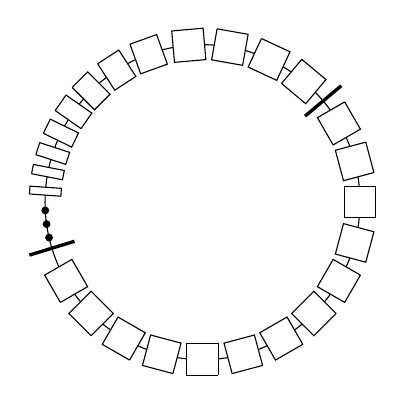
\begin{tikzpicture}
		\draw (0,0) ellipse [radius=2cm];
		\foreach \angle / \width in {
			0/1, 15/1, 30/1,
			50/1, 65/1, 80/1, 95/1,
			110/0.9, 123/0.8, 135/0.7, 145/0.6, 154/0.5, 162/0.4, 169/0.3, 176/0.25,
			345/1, 330/1, 315/1, 300/1, 285/1, 270/1, 255/1, 240/1, 225/1, 210/1
		}
		\path [rotate=\angle,xshift=2cm,yscale=\width, draw=black, fill=white] (0,0) +(0.2,0.2) -- +(0.2,-0.2) -- +(-0.2,-0.2) -- +(-0.2,0.2) -- +(0.2,0.2);
		\foreach \angle in {183, 188, 193}
		\draw (\angle:2cm) node [fill,circle, inner sep=1pt] {};
		\draw [very thick] (40:1.7) -- (40:2.3) (197:1.7) -- (197:2.3);
	\end{tikzpicture}

\end{document}